\section{Architectural Decisions, Layers and Tiers}

\subsection{Solution Strategy}
It includes the fundamental decisions and solutions strategies that shape the system's architecture. These decisions form the cornerstones for your architecture. They are the basis for many other detailed decisions or implementation rules.

These include:
\begin{itemize}
  \item Technology decisions
  \item Decisions about the top-level decomposition of the system, e.g. usage of an architectural pattern or design pattern
  \item Decisions on how to achieve key quality goals
  \item Relevant organizational decisions, e.g. selecting a development process or delegating certain tasks to third parties.
\end{itemize}

\subsection{Architectural Decisions (AD)}
Architectural decisions capture key design issues and the rationale behind chosen solutions. They are conscious design decisions concerning a software-intensive system as a whole or one or more of its core components and connectors in any given view. The outcome of architectural decisions influences the system’s nonfunctional characteristics including its software quality attributes.

An \textbf{Architectural Decision Record (ADR)} captures a single AD, such as often done when writing personal notes or meeting minutes; the collection of ADRs created and maintained in a project constitute its decision log.

\paragraph{Y-Template} \hfill \\
Writing formal ADD can be hard and time consuming. Also it is a good idea to make them accessible to the developer team, to make sure they can be reread again and also made sure they are not forgotten. The Y-Model in figure \ref{fig:ymodel} from ABB provides a template to write ADDs.

\begin{figure}[H]
  \center
  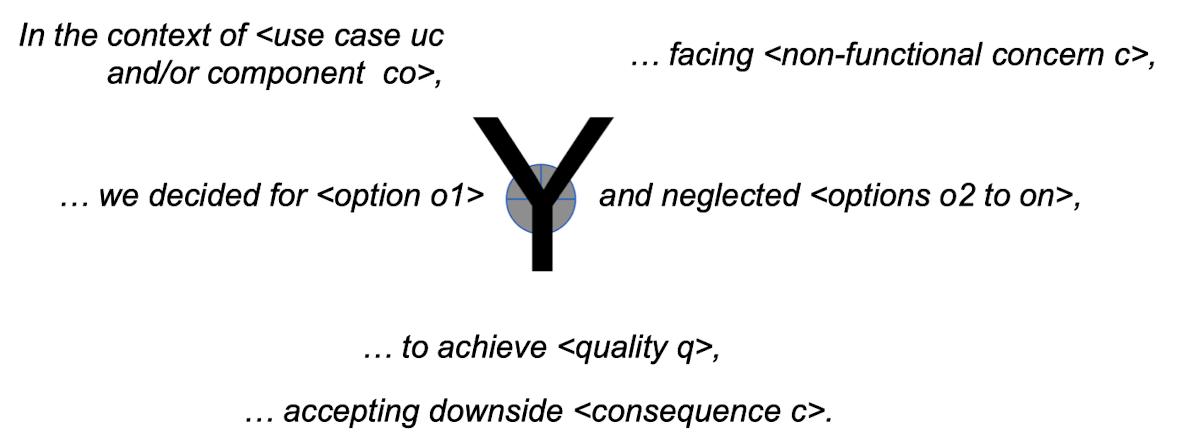
\includegraphics[width=0.65\textwidth]{architecturaldesigndecision}
  \caption{Architectural Design Decision}
  \label{fig:ymodel}
\end{figure}

\textit{Example ADR 1 with the Y-Model:}
In the context of the frontend facing the NFR fast response time, we decided for Deck, a non-distributed presentation layer and neglected ExpressJS to achieve fast response times and accepting the heavier load on the user machines.

\textit{Example ADR 2 with the Y-Model:}
In the context of the order management scenario at T,
facing the need to process customer orders synchronously, without loosing
any messages,
we decided to apply the Messaging pattern and the RPC pattern
and neglected File Transfer, Shared Database, no physical distribution (local calls)
to achieve guaranteed delivery and request buffering when dealing with
unreliable data sources
accepting that follow
on detailed design work has be performed and that
we need to select, install, and configure a message oriented middleware
provider.

\subsection{Logical Layering}
Most of the time we have a system needs to be segmented due to its size and specialisation. The problem is, that we need to have a system design, that supports a mixture of tasks on different levels. The solution we have in software engineering is, we organise the system into cohesive layers that are stacked on top of each other. This approach is called the Layers Pattern and are typically applied twice: \textbf{logical and physical} view.

Two of the big decisions in Solution Strategy is on choosing layers and tiers. It is important to understand the distinction between layers and tiers.

\begin{description}
  \item [Layers] describe the logical groupings of the functionality and components in an application
  \item [Tiers]  describe the physical distribution of the functionality and components on separate servers, computers, networks, or remote locations
\end{description}

\begin{figure}[h!]
  \center
  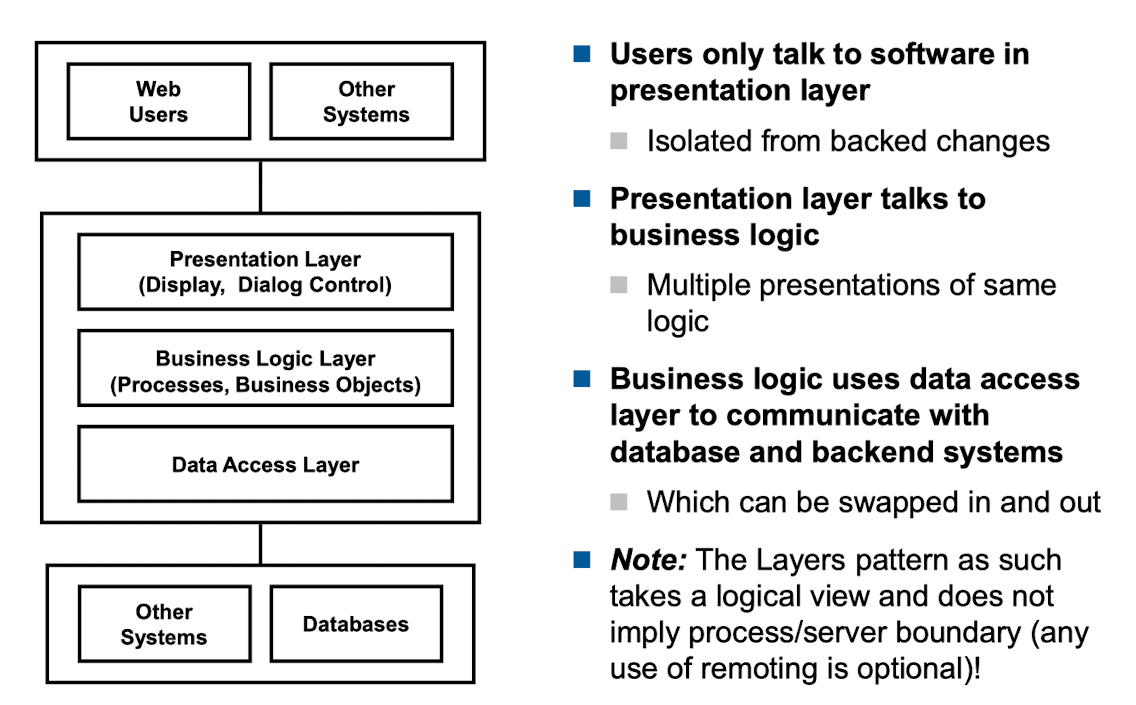
\includegraphics[width=0.75\textwidth]{layerpattern}
  \caption{Layer Pattern}
\end{figure}

\subsection{Distribution Patterns}
The Problem is now, how do I partition an application into a number of client and server components so that my users' functional and non-functional requirements are met?

To distribute an information system by assigning client and server roles to the components of the layered architecture we have the choice of several distribution styles. Figure \ref{fig:patternlanguage} shows the styles which build the pattern language which are called \textbf{Client/Server Cuts}.

\begin{figure}[H]
  \center
  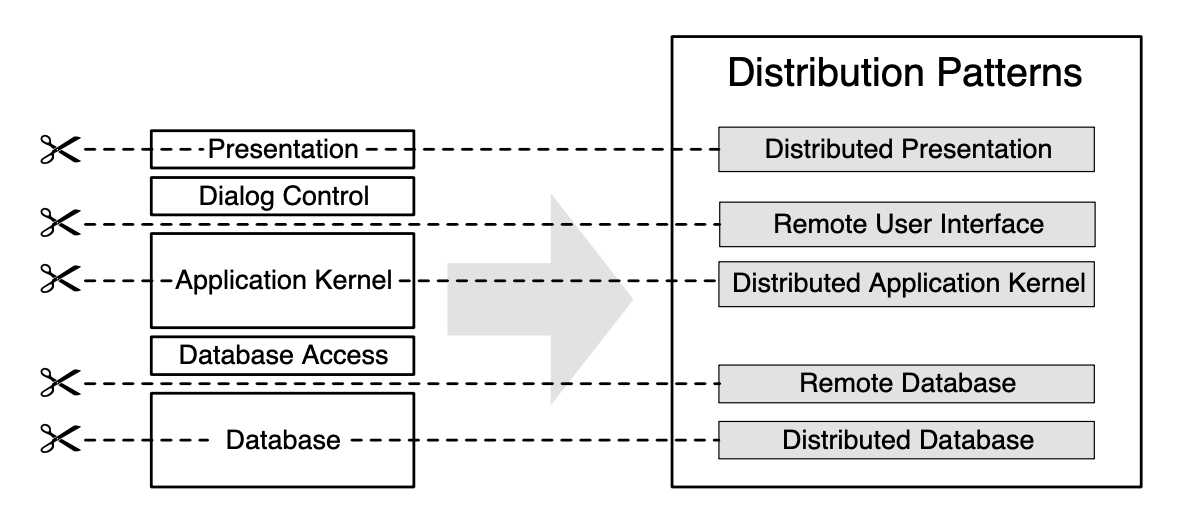
\includegraphics[width=0.75\textwidth]{architecturepattern}
  \caption{Overview of the patterns resulting from different client/server cuts}
  \label{fig:patternlanguage}
\end{figure}


To take a glance at the pattern language we give an abstract for each pattern:¨
\begin{description}
  \item [Distributed Presentation] This pattern partitions the system within the presentation component. One part of the presentation component is packaged as a distribution unit and is processed separately from the other part of the presentation which can be packaged together with the other application layers. This pattern allows of an easy implementation and very thin clients.
  \item [Remote User Interface] Instead of distributing presentation functionality the whole user interface becomes a unit of distribution and acts as a client of the application kernel on the server side.
  \item [Distributed Application Kernel] The pattern splits the application kernel into two parts which are processed separately. This pattern becomes very challenging if transactions span process boundaries (distributed transaction processing).
  \item [Remote Database]  The database is a major component of a business information system with special requirements on the execution environment. Sometimes, several applications work on the same database. This pattern locates the database component on a separate node within the system’s network.
  \item [Distributed Database] The database is decomposed into separate database components, which interact by means of interprocess communication facilities. With a distributed data- base an application can integrate data from different database systems or data can be stored more closely to the location where it is processed.
\end{description}

There are pros and cons for using different distribution patterns. Take a look at figure \ref{fig:dpatternsdiscussion}, where they are explained.

\begin{figure}[H]
  \center
  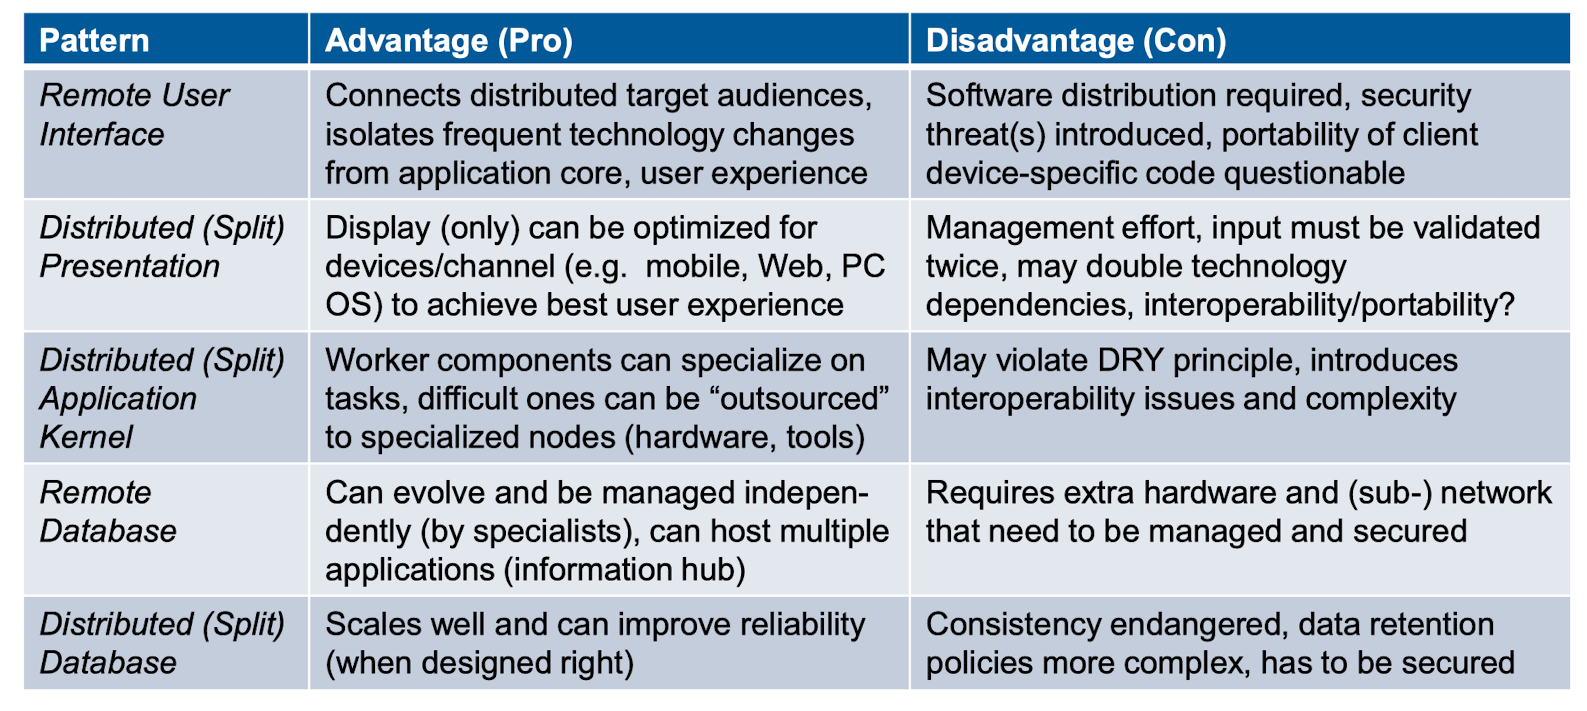
\includegraphics[width=0.9\textwidth]{distributionpatternsdiscussion}
  \caption{Pros and Cons of Distribution Patterns}
  \label{fig:dpatternsdiscussion}
\end{figure}

Each pattern presents a partial distribution view of the application architecture and maps this to a physical system structure. As a solution addresses only a part of the application components the whole distribution model may result from applying more than one distribution pat- tern. Instances of application components can „live“ on different nodes of the technical architecture, because of components being part of more than one distribution unit or distribution units mapped to different nodes.

\begin{figure}[H]
  \center
  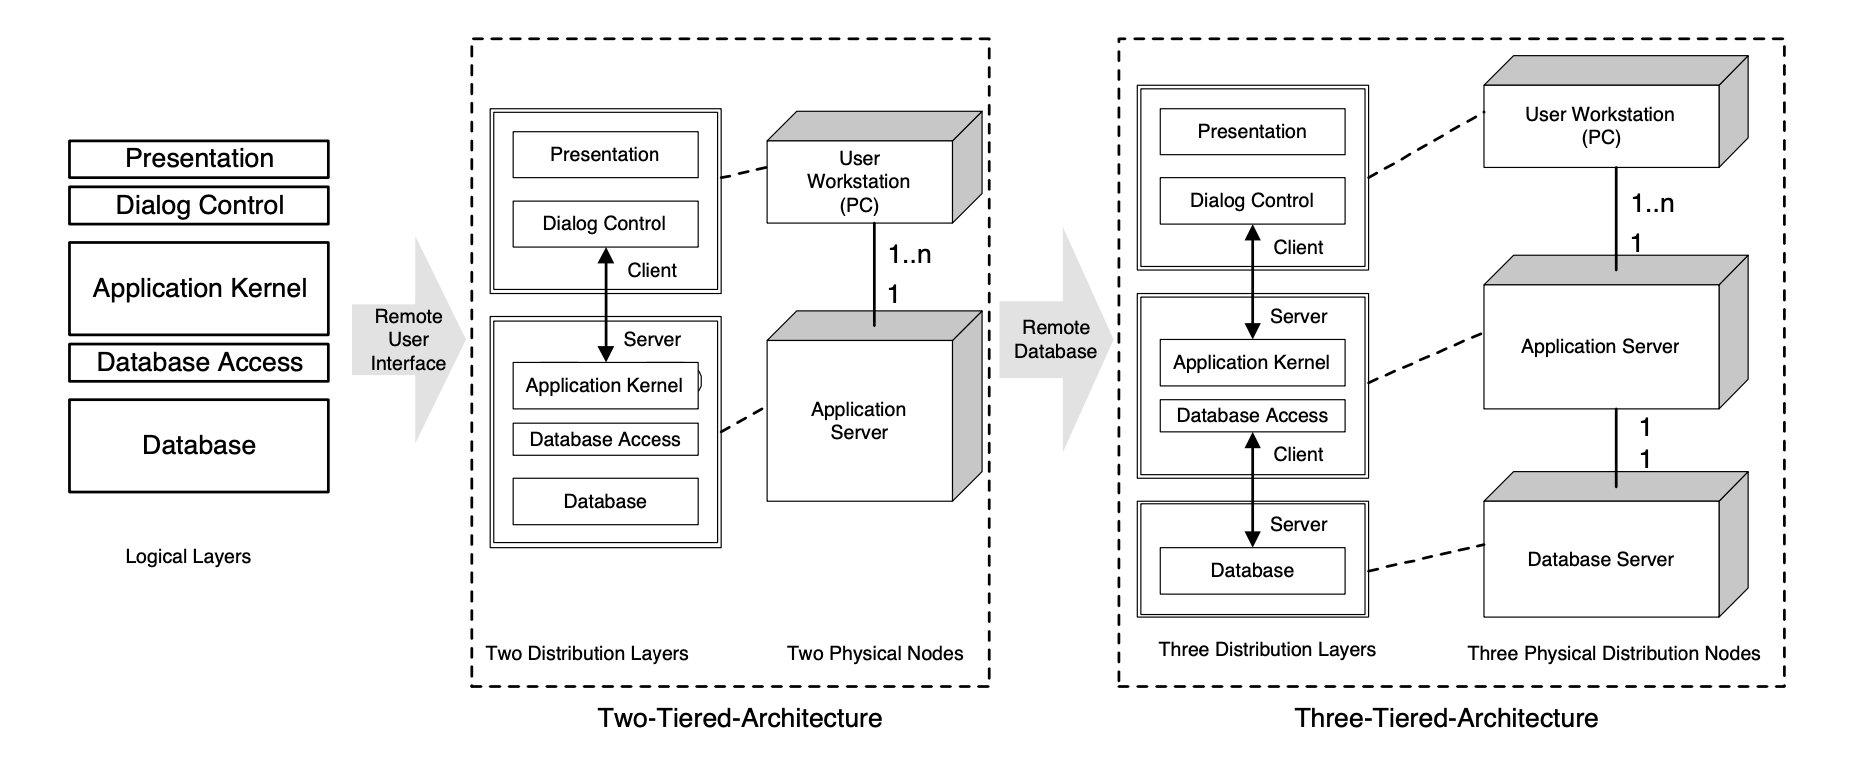
\includegraphics[width=\textwidth]{distributionpatterns.png}
  \caption{Building a Three-Tiered-Architecture applying the Remote User Interface pattern and the Remote Database pattern}
\end{figure}

\begin{figure}[H]
  \center
  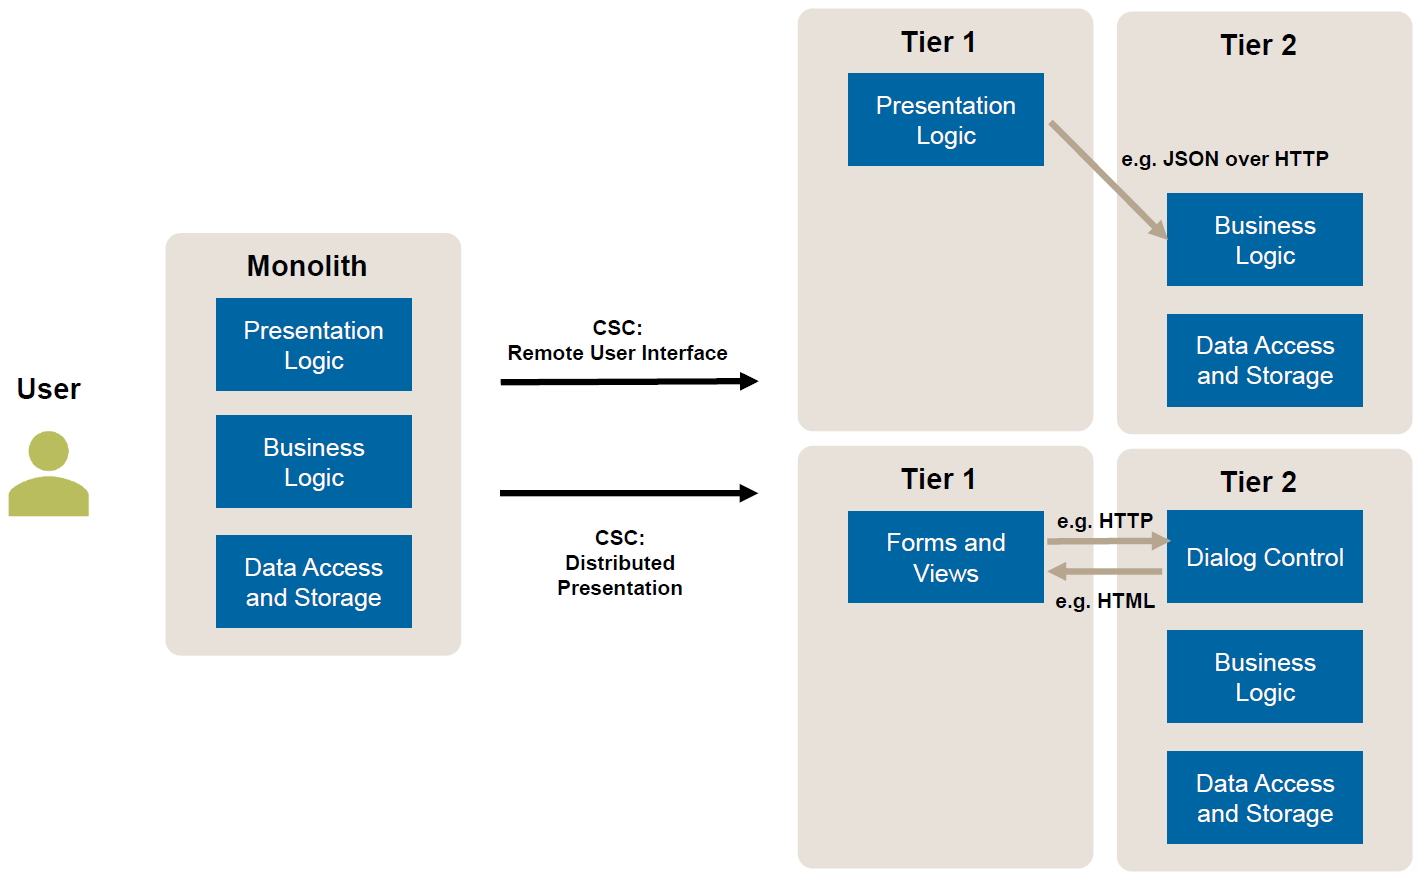
\includegraphics[width=0.75\textwidth]{client-vs-server-side-rendering.png}
  \caption{Two-Tier-Architecture with Client-Side-Rendering and Server-Side-Rendering}
\end{figure}

\subsection{arc42}
arc42 is an open source documentation template and is based on practical experience of many systems in various domains, from information and web systems, real-time and embedded to business intelligence and data warehouses. arc42 answers the following two questions in a pragmatic way and can be tailored to your specific needs: \textit{What should you document/communicate about your architecture?,  How should you document/communicate?}.

\begin{figure}[H]
  \center
  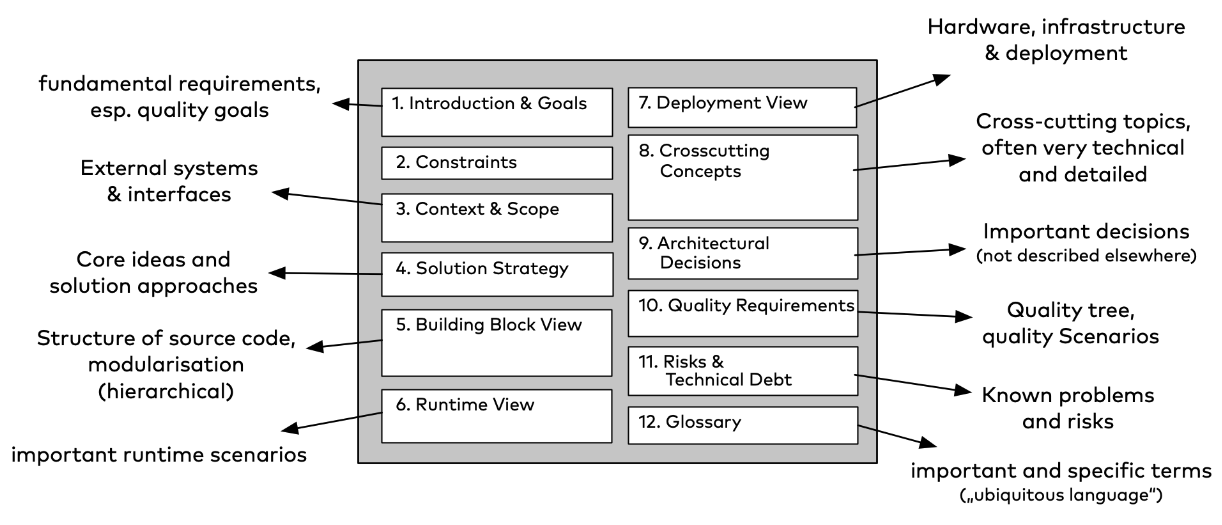
\includegraphics[width=\textwidth]{arc42}
  \caption{arc42 Overview}
\end{figure}
